\documentclass[11pt]{article}

\usepackage[margin=1in]{geometry}
\usepackage{amsmath, amssymb}
\usepackage{graphicx}
\usepackage{booktabs}
\usepackage{hyperref}
\usepackage{xcolor}
\usepackage{caption}
\usepackage{subcaption}
\usepackage{tikz}
\usetikzlibrary{arrows.meta, positioning, calc}

\title{Model Comparison on the Cylinder Graph HMM}
\author{Claude \& C. L.}
\date{\today}

\begin{document}
\maketitle

%----------------------------------------------------------------------
\section{Introduction}
%----------------------------------------------------------------------

\newcommand{\lcq}[1]{\textcolor{red}{#1}}

A Hidden Markov Model (HMM) is a stochastic process in which an
unobservable (hidden) Markov chain $\{S_t\}$ over a finite state space
generates an observed sequence $\{X_t\}$ through state-dependent
emission distributions.  At each time step the chain transitions from
state $s$ to state $s'$ with probability $T(s, s')$ and emits an
observable token $v$ with probability $O(v \mid s')$.  Because the
hidden states are not directly accessible, a predictor must infer the
latent state from the history of observations alone.

In this report we study how small transformer language models learn to
perform this inference on a structured HMM whose hidden-state graph has
the topology of a discrete cylinder (Section~\ref{sec:hmm}).  We first
establish information-theoretic baselines---the entropy rate, the
Bayes-optimal predictor at finite context, and $n$-gram
models---against which transformer performance can be measured
(Section~\ref{sec:baselines}).  We then describe the transformer
architectures and training procedure (Section~\ref{sec:transformers}),
present results on scaling, architecture, and embedding structure
(Section~\ref{sec:results}), and conclude with open questions
(Section~\ref{sec:summary}).

%----------------------------------------------------------------------
\section{The Cylinder Graph HMM}\label{sec:hmm}
%----------------------------------------------------------------------

We consider an HMM whose hidden-state graph has the topology of a
discrete cylinder with \emph{width} $n = 6$ (nodes per level) and
\emph{depth} $D = 3$ (number of levels), giving
$n \times D = 18$ hidden states in total.

\subsection{Transition structure}

Each level $l \in \{0, 1, 2\}$ contains $n = 6$ nodes arranged in a
ring.  From a node $(l, j)$ at depth $l$ and angular position $j$ the
chain can jump to three neighbours:
\begin{itemize}
  \item \textbf{Nearest neighbour (NN):} $(l,\, j{+}1 \bmod n)$ with
        weight $w$, where $w \sim \mathrm{Uniform}(0,\, 1{-}p)$;
  \item \textbf{Next-nearest neighbour (NNN):} $(l,\, j{+}2 \bmod n)$
        with weight $1 - p - w$;
  \item \textbf{Next layer:} $((l{+}1) \bmod D,\, j)$ with fixed
        probability $p = 0.1$.
\end{itemize}
The intra-layer weights $w$ are drawn independently for each node from
$\mathrm{Uniform}(0,\, 1{-}p)$ once at initialisation (seed~42) and
held fixed thereafter.  The inter-layer probability $p$ controls how
often the chain cycles through the depth levels.


\subsection{Emission structure}

The vocabulary has $|V| = D \times K = 3 \times 16 = 48$ tokens,
partitioned into three clusters of 16 tokens each (one cluster per depth
level).  Each hidden state at depth $l$ emits tokens only from cluster
$l$, with emission probabilities drawn from a symmetric Dirichlet
distribution with concentration parameter $\alpha = 0.3$.  The small
$\alpha$ makes the per-state distributions sparse, so different states
at the same depth emit noticeably different token profiles.

%----------------------------------------------------------------------
\section{Information-Theoretic Baselines}\label{sec:baselines}
%----------------------------------------------------------------------

\subsection{Entropy rate}\label{sec:entropy-rate}

The \emph{entropy rate} of a stationary stochastic process $\{X_t\}$ is
\begin{equation}
  h \;=\; \lim_{T \to \infty} \frac{1}{T} H(X_1, \dots, X_T)
    \;=\; \lim_{T \to \infty} H(X_T \mid X_1, \dots, X_{T-1}).
\end{equation}
For the second equality, we have used the chain rule of entropy. The entropy rate of a stochastic process is the irreducible uncertainty per token for a predictor with access to the infinite past, and therefore serves as the information-theoretic lower bound on the cross-entropy loss achievable by any model.

For an HMM with transition matrix $T$ and emission matrix $O$, the
entropy rate can be estimated empirically by generating a long sequence
$(x_1, \dots, x_N)$, running the forward algorithm to compute the
predictive probabilities $P(x_t \mid x_1, \dots, x_{t-1})$, and
averaging:
\begin{equation}
  \hat{h} \;=\; -\frac{1}{N - N_{\mathrm{burn}}}
    \sum_{t=N_{\mathrm{burn}}+1}^{N} \log P(x_t \mid x_1, \dots, x_{t-1}),
\end{equation}
where the first $N_{\mathrm{burn}}$ tokens are discarded to allow the
belief state to converge from an arbitrary prior.  For the cylinder
graph HMM with the parameters specified above, this yields \(\hat{h} \approx 2.44\) nats/token.

\subsection{Bayes-optimal loss at finite context}\label{sec:bayes-optimal}

The entropy rate is the minimum achievable loss for a predictor with
access to the \emph{infinite} past.  A transformer with context window $T$,
however, can only condition on the most recent $T$ tokens.  To
disentangle the loss due to \emph{finite context} from the loss due to
\emph{limited model capacity}, we compute the Bayes-optimal next-token
loss at finite context: the best any predictor can do when restricted to
a window of length~$k$.

Let $\{X_t\}$ be the observed token process generated by the HMM with
hidden states $\{S_t\}$, transition--emission matrices
$E[v,s,s'] = P(X_t{=}v,\, S_t{=}s' \mid S_{t-1}{=}s)$, and stationary
distribution $\pi$.

Given a context window $(x_1,\dots,x_k)$, the Bayes-optimal prediction
for the next token is
\begin{equation}\label{eq:bayes-pred}
  P(X_{k+1}{=}v \mid x_1,\dots,x_k)
  \;=\; \sum_{s,s'} \alpha_k(s)\, E[v,s,s'],
\end{equation}
where $\alpha_k$ is the posterior (belief state) over hidden states after
processing the context. The belief state is computed recursively via the forward algorithm.
Initialise from the stationary prior $\alpha_0(s) = \pi(s)$.  Upon
observing token $x_t$, update:
\begin{equation}\label{eq:forward}
  \tilde{\alpha}_t(s')
  \;=\; \sum_s \alpha_{t-1}(s)\, E[x_t, s, s'],
  \qquad
  \alpha_t(s') = \frac{\tilde{\alpha}_t(s')}
                      {\displaystyle\sum_{s''}\tilde{\alpha}_t(s'')}.
\end{equation}
The normalising constant $Z_t = \sum_{s'}\tilde{\alpha}_t(s')$ equals
the predictive probability $P(x_t \mid x_1,\dots,x_{t-1})$, so the
conditional log-likelihood of the context decomposes as
$\log P(x_1,\dots,x_k) = \sum_{t=1}^{k} \log Z_t$.

After $k$ update steps the belief $\alpha_k$ encodes all information
that the context provides about the current hidden state.  Plugging it
into Eq.~\eqref{eq:bayes-pred} yields the Bayes-optimal predictive
distribution and hence the minimum achievable loss at context length~$k$:
\begin{equation}\label{eq:Lstar}
  L^{*}(k)
  \;=\; \mathbb{E}\!\Bigl[
    -\log P\bigl(X_{k+1} \mid X_1,\dots,X_k\bigr)
  \Bigr],
\end{equation}
where the expectation is over sequences drawn from the HMM\@.

For a \emph{fixed} context window, each length-$k$ chunk is treated
independently: the belief is reset to $\pi$ at the start of every
window.  This is exactly the information available to a transformer with
context length~$k$.  For the \emph{infinite-context} baseline, the
forward algorithm runs over the entire sequence without resetting, so
the belief accumulates information from arbitrarily far in the past.
The difference
\begin{equation}
  \Delta(k) \;=\; L^{*}_{\text{fixed}}(k) - L^{*}_{\infty}
\end{equation}
isolates the cost of the finite context window.  As $k$ grows beyond the
mixing time of the chain, $\Delta(k) \to 0$.

The cross-entropy loss of a trained transformer $\hat{L}$ can therefore
be decomposed as
\begin{equation}\label{eq:loss-decomp}
  \underbrace{\hat{L}}_{\text{transformer loss}}
  \;=\; \underbrace{h\vphantom{\hat{L}}}_{\text{entropy rate}}
  \;+\; \underbrace{\Delta(k)\vphantom{\hat{L}}}_{\text{finite-context cost}}
  \;+\; \underbrace{D_{\mathrm{KL}}\vphantom{\hat{L}}}_{\text{model capacity gap}},
\end{equation}
where $D_{\mathrm{KL}} = \hat{L} - L^{*}_{\text{fixed}}(k) \ge 0$
measures the sub-optimality of the transformer relative to the
Bayes-optimal predictor at the same context length.

\subsection{$N$-gram baseline}\label{sec:ngram-baseline}

An $n$-gram model estimates the next-token distribution by conditioning
on a fixed-length context of $n{-}1$ preceding tokens.  The maximum
likelihood estimate is
\begin{equation}\label{eq:ngram-mle}
  \hat{P}_{\text{MLE}}(w \mid w_{t-n+1},\dots,w_{t-1})
  \;=\; \frac{C(w_{t-n+1},\dots,w_{t-1},\, w)}
             {C(w_{t-n+1},\dots,w_{t-1})},
\end{equation}
where $C(\cdot)$ denotes the count of the $n$-gram (or $(n{-}1)$-gram
context) in the training corpus.  When a context has never been observed,
we back off to shorter contexts until a match is found (see
Appendix~\ref{app:ngram-details} for smoothing and backoff details).
The implementation is in \texttt{src/ngram\_baseline.py}.

\subsection{Summary of baselines}

Table~\ref{tab:baselines} summarises the theoretical and empirical
baselines.

\begin{table}[htbp]
  \centering
  \begin{tabular}{l r l}
    \toprule
    Baseline & Loss (nats) & Description \\
    \midrule
    Entropy rate $h$ & $\approx 2.44$ & Infinite-context lower bound \\
    Bayes-optimal $L^{*}(k{=}16)$ & $\approx 2.47$ & Best fixed-context ($k{=}16$) predictor \\
    Best $n$-gram (trigram) & $2.57$ & Best count-based model (test CE) \\
    Bigram & $2.67$ & Single-token context baseline \\
    Unigram & $3.65$ & No context (marginal frequencies) \\
    \bottomrule
  \end{tabular}
  \caption{Information-theoretic and count-based baselines for the
           cylinder graph HMM\@.  The finite-context cost
           $\Delta(16) \approx 0.03$\,nats is small, indicating that the
           context window $k = 16$ is already sufficient for near-optimal
           inference.}
  \label{tab:baselines}
\end{table}

%----------------------------------------------------------------------
\section{Transformer Architectures}\label{sec:transformers}
%----------------------------------------------------------------------

We train causal transformer language models (implemented via
TransformerLens \texttt{HookedTransformer}) to predict the next token in
sequences of length $T = 16$ generated by the cylinder HMM.

The hyperparameter sweep covers:
\begin{center}
\begin{tabular}{ll}
  \toprule
  Hyperparameter & Values \\
  \midrule
  Number of layers $L$        & 2, 4 \\
  Embedding dimension $d$     & 4, 8, 16, 32, 48, 64 \\
  Number of heads $H$         & 1, 2, 4 \\
  Architecture                & attention-only, full (attention + MLP) \\
  Normalisation               & none, LayerNorm \\
  \bottomrule
\end{tabular}
\end{center}
All models use ReLU activations, tied input/output embeddings, and
$d_{\mathrm{mlp}} = 4d$ for full architectures.  Training uses AdamW
($\beta_1 = 0.9$, $\beta_2 = 0.999$, weight decay $0.01$, learning rate
$10^{-3}$) with batch size 128 for 10 epochs.  A total of 135 models
were trained on a dataset of ${\sim}\,618\text{k}$ sequences
($10^7$ tokens).

%----------------------------------------------------------------------
\section{Results}\label{sec:results}
%----------------------------------------------------------------------

\subsection{Model size vs.\ validation loss}

Figure~\ref{fig:model-comparison} plots the best validation loss
achieved by each model against its parameter count.

\begin{figure}[htbp]
  \centering
  \begin{subfigure}[t]{0.48\textwidth}
    \centering
    
\includegraphics[width=\textwidth]{model_comparison.png}
    \caption{Validation loss vs.\ parameter count.  Circles: attention-only;
             squares: full (attention + MLP).  Blue: LayerNorm; red: no
             normalisation.  Dashed lines mark the entropy rate
             $h \approx 2.44$\,nats/token, the Bayes-optimal loss
             $L^{*}(k{=}16) \approx 2.47$\,nats, and the best $n$-gram
             baseline (trigram, $2.57$\,nats).}
    \label{fig:model-comparison-abs}
  \end{subfigure}
  \hfill
  \begin{subfigure}[t]{0.48\textwidth}
    \centering
    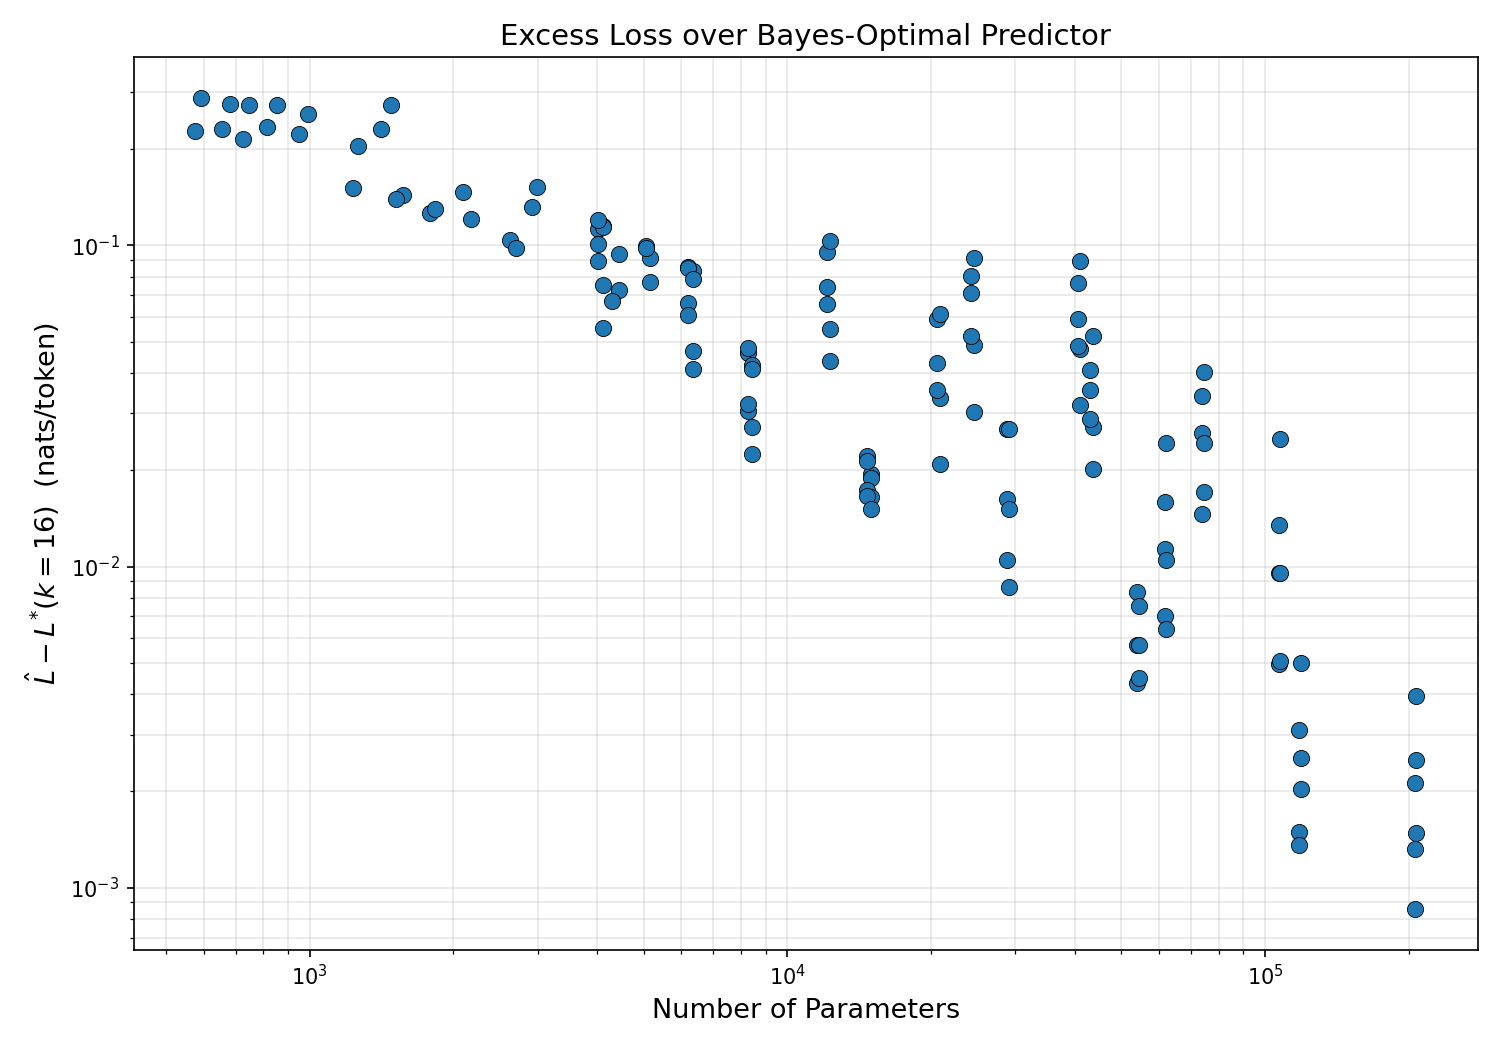
\includegraphics[width=\textwidth]{excess_loss_loglog.png}
    \caption{Excess loss $\hat{L} - L^{*}(k{=}16)$ on a log--log scale.
             All architectural distinctions are suppressed to highlight
             the overall scaling trend with model size.}
    \label{fig:model-comparison-excess}
  \end{subfigure}
  \caption{Model size versus validation loss for 135 transformer
           configurations on the Cylinder Graph HMM\@.
           (a)~Absolute validation loss.
           (b)~Excess loss over the Bayes-optimal predictor at context
           length~$k = 16$.}
  \label{fig:model-comparison}
\end{figure}

Validation loss decreases roughly log-linearly with parameter count up
to ${\sim}10^5$ parameters, after which gains diminish.  At every
scale, full transformers (with MLP layers) outperform their
attention-only counterparts, and all top-10 models use $L = 4$ layers.
LayerNorm has a negligible effect compared to architecture and scale.
The best model (L4, $d{=}64$, $H{=}4$, full, no-LN; ${\sim}206$k
parameters) reaches ${\approx}\,2.473$\,nats/token.  By the
decomposition in Eq.~\eqref{eq:loss-decomp}, most of the
$0.034$\,nat gap above the entropy rate is attributable to the finite
context window ($\Delta(16) \approx 0.03$\,nats), leaving only
${\sim}0.004$\,nats of model capacity gap.

\subsection{$N$-gram comparison}

Table~\ref{tab:ngram} reports the training and test cross-entropy loss for
$n$-gram orders 1 through 6 (without regularisation; see
Appendix~\ref{app:ngram-details} for smoothed results).

\begin{table}[htbp]
  \centering
  \begin{tabular}{r r r r}
    \toprule
    $n$ & Train CE & Test CE & \# Contexts \\
    \midrule
    1 & 3.654 & 3.652 &           1 \\
    2 & 2.667 & 2.669 &          48 \\
    3 & 2.551 & 2.566 &       1\,540 \\
    4 & 2.470 & 2.832 &      39\,531 \\
    5 & 2.236 & 4.781 &     443\,415 \\
    6 & 1.713 & 8.618 &   1\,953\,864 \\
    \bottomrule
  \end{tabular}
  \caption{$N$-gram cross-entropy (nats/token) without regularisation.
           For $n \geq 4$, test loss diverges due to overfitting.
           The best test performance is the trigram ($n = 3$).}
  \label{tab:ngram}
\end{table}

The largest drop in cross-entropy occurs from the unigram to the bigram
($3.65 \to 2.67$ nats), reflecting the strong first-order correlations
induced by the HMM's clustered emission structure: observing a single
token already reveals the current depth level, narrowing the effective
vocabulary from~48 to~16.  The trigram provides a modest further gain,
approaching the Bayes-optimal loss.  The best $n$-gram model (trigram,
test CE $= 2.57$) is outperformed by transformers with embedding
dimension $d \ge 16$, suggesting that these models learn to approximate
belief-state inference beyond simple token co-occurrence statistics.
Conversely, very small transformers ($d = 4$) fail to beat the trigram,
indicating that a minimum model capacity is needed before the
transformer can surpass what a count table captures directly.

\subsection{Embedding structure}

Figure~\ref{fig:embedding} shows the cosine-similarity matrix and
$\ell_2$ norms of the learned token-embedding vectors from a
representative model.  The $3 \times 3$ block structure in the
similarity matrix directly mirrors the depth-level clustering of the
vocabulary: tokens within the same depth cluster are mapped to similar
embedding directions, while cross-cluster pairs are near-orthogonal or
anti-correlated.  This confirms that the model discovers the latent
depth structure without supervision.

\begin{figure}[htbp]
  \centering
  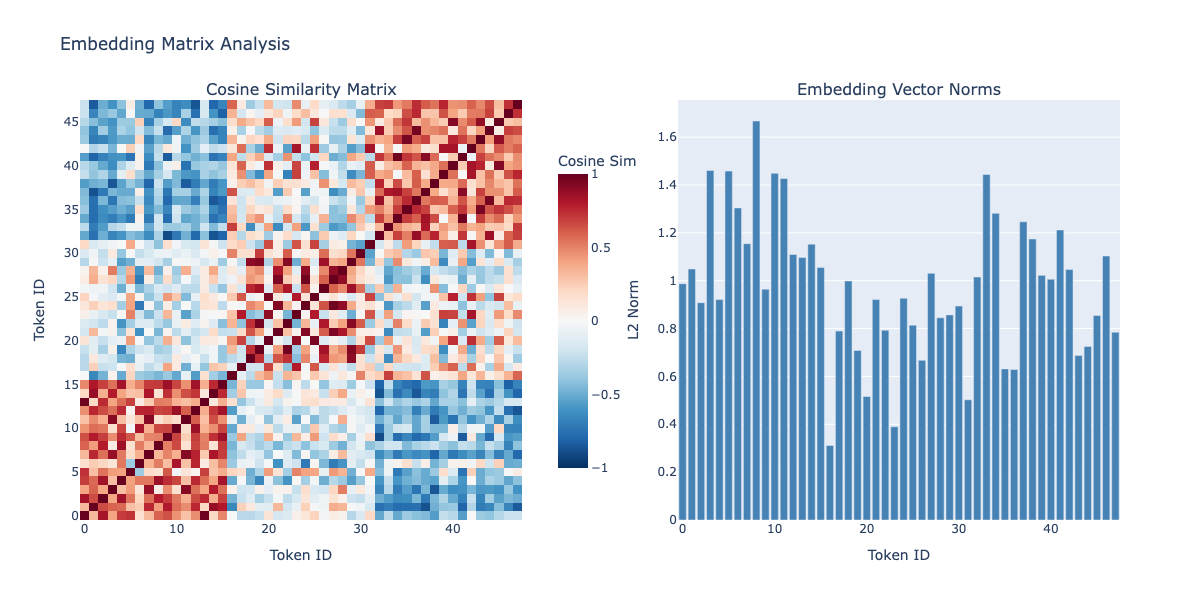
\includegraphics[width=0.85\textwidth]{newplot.png}
  \caption{Left: cosine similarity matrix of the $48 \times d$ embedding
           matrix.  The visible $3 \times 3$ block structure corresponds
           to the three depth levels.  Right: $\ell_2$ norm of each
           token's embedding vector.}
  \label{fig:embedding}
\end{figure}

\paragraph{Cluster similarity across architectures}
To quantify how consistently the embedding geometry reflects the
depth-level structure, we compute the cosine similarity between cluster
centroids across all 135 trained models.  For each model we extract the
embedding matrix $W_E \in \mathbb{R}^{48 \times d}$ and compute three
centroids
\begin{equation}
  \mathbf{c}_l = \frac{1}{16}\sum_{v=16l}^{16l+15} W_E[v,:],
  \qquad l \in \{0,1,2\},
\end{equation}
followed by the three pairwise cosine similarities
$\mathrm{sim}(\mathbf{c}_0, \mathbf{c}_1)$,
$\mathrm{sim}(\mathbf{c}_0, \mathbf{c}_2)$, and
$\mathrm{sim}(\mathbf{c}_1, \mathbf{c}_2)$.

Figure~\ref{fig:cluster-sim} shows these similarities as a function of
validation loss.  All three pairs are predominantly negative
(mean $\approx -0.4$), confirming that the learned embeddings separate
the three depth clusters into roughly opposing directions in embedding
space.  Models that achieve low validation loss (left side of the plot)
cluster tightly in the range $-0.35$ to $-0.50$, while poorly
performing models exhibit much higher variance---some cluster pairs even
become positively correlated.  This suggests that learning to separate
the depth clusters in embedding space is necessary for good predictive
performance, but the degree of separation saturates once the model is
sufficiently expressive.

\begin{figure}[htbp]
  \centering
  \begin{subfigure}[t]{0.48\textwidth}
    \centering
    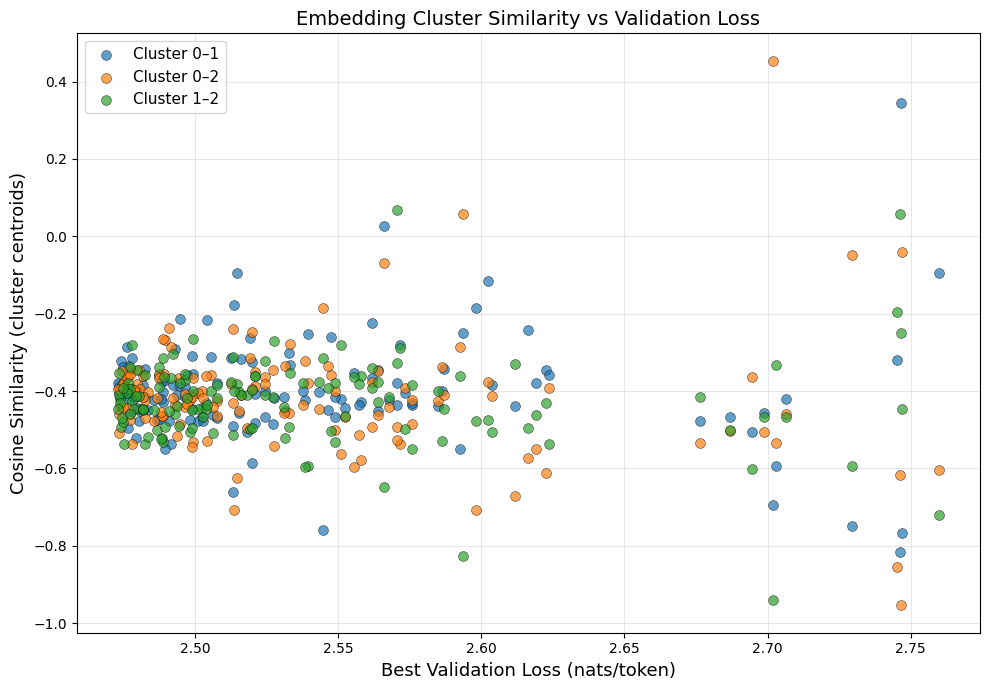
\includegraphics[width=\textwidth]{figures/embedding_cluster_similarity_raw.png}
    \caption{All three pairwise cosine similarities between cluster
             centroids, plotted for each of the 135 trained models.
             Poorly performing models show high variance, with some
             cluster pairs becoming positively correlated.}
    \label{fig:cluster-sim-raw}
  \end{subfigure}
  \hfill
  \begin{subfigure}[t]{0.48\textwidth}
    \centering
    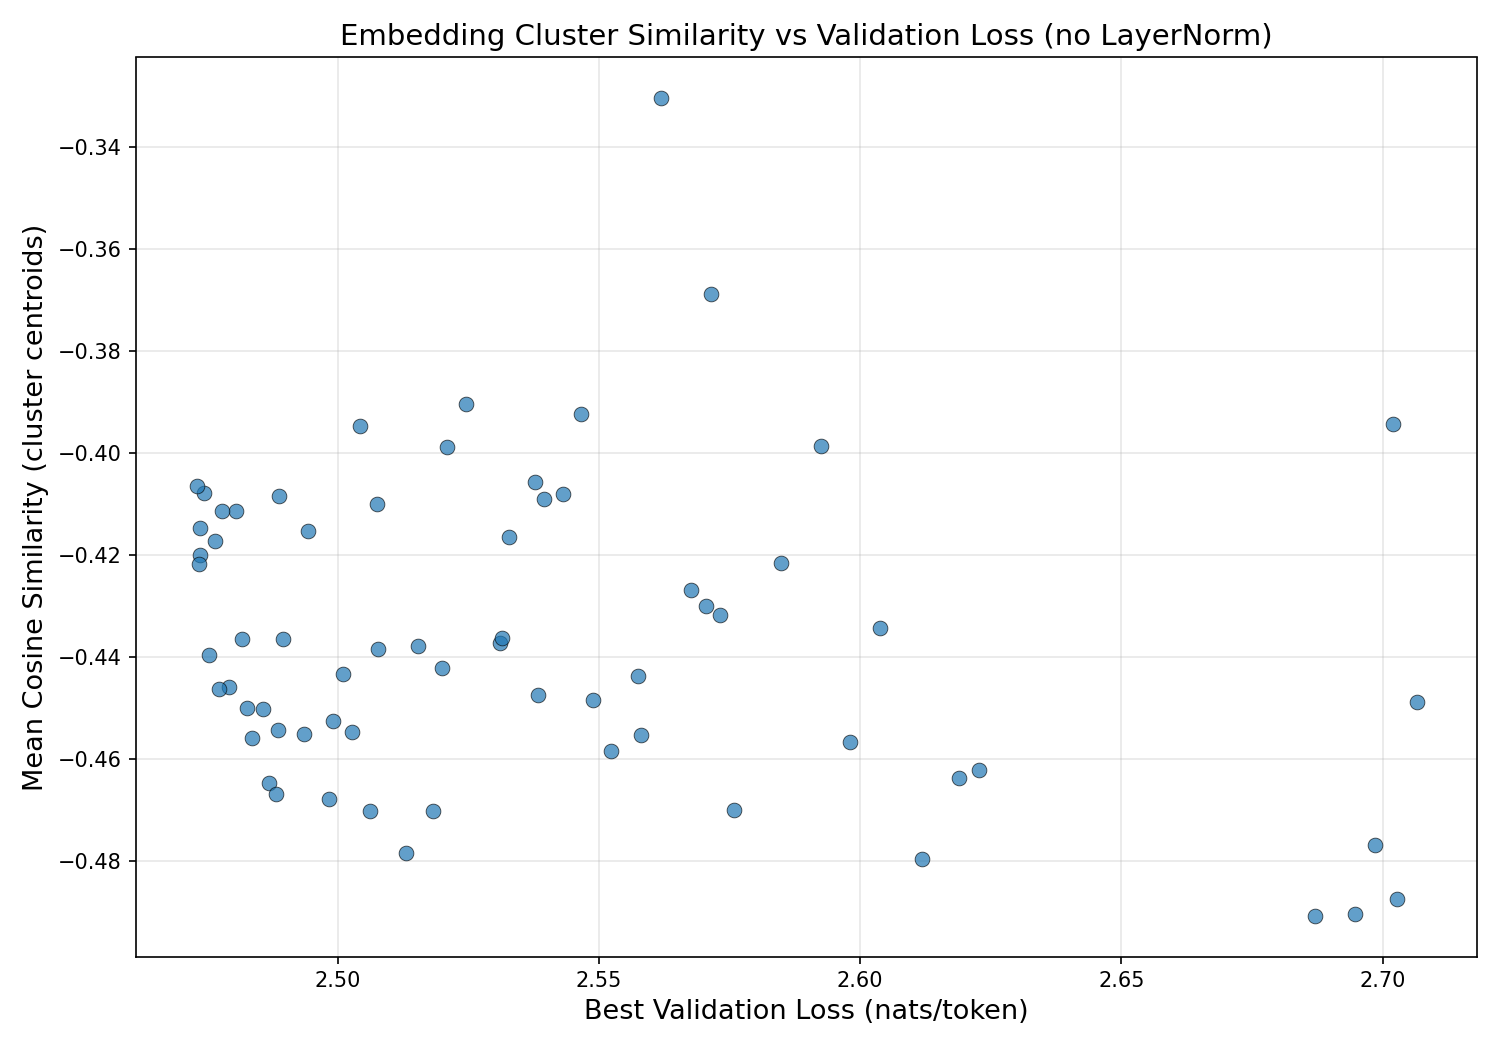
\includegraphics[width=\textwidth]{figures/embedding_cluster_similarity.png}
    \caption{Mean of the three pairwise similarities per model,
             restricted to architectures without LayerNorm (67~models).
             The trend is flat, with most models in $[-0.49, -0.35]$.}
    \label{fig:cluster-sim-mean}
  \end{subfigure}
  \caption{Cosine similarity between depth-cluster centroids of the
           embedding matrix versus best validation loss.
           (a)~Per-pair similarities for all models.
           (b)~Mean similarity for noLN models only.}
  \label{fig:cluster-sim}
\end{figure}

%----------------------------------------------------------------------
\section{Summary and Open Questions}\label{sec:summary}
%----------------------------------------------------------------------

The cylinder graph HMM provides a controlled testbed for studying how
transformers learn to perform approximate Bayesian filtering over a
structured latent space.  Larger, deeper, full-architecture models
approach but do not reach the entropy rate, suggesting fundamental
limits tied to the autoregressive architecture and finite context.

Open directions include:
\begin{itemize}
  \item Characterising the belief-state geometry learned by the residual
        stream (cf.\ the fractal structure observed in the belief-state
        notebooks).
  \item Ablation studies on context length to quantify the loss
        attributable to finite $T$.
  \item Mechanistic interpretability of attention heads---do specific
        heads specialise in tracking depth transitions versus intra-layer
        dynamics?
\end{itemize}


%======================================================================
\appendix
%======================================================================

\section{$N$-gram Smoothing and Backoff Details}\label{app:ngram-details}

\paragraph{Laplace smoothing}
The MLE assigns zero probability to any $n$-gram unseen in training,
producing infinite cross-entropy on test data.  Laplace (add-$k$)
smoothing regularises the estimate by adding $k$ pseudocounts to every
possible continuation:
\begin{equation}\label{eq:ngram-smooth}
  \hat{P}_{k}(w \mid \mathbf{c})
  \;=\; \frac{C(\mathbf{c},\, w) + k}
             {C(\mathbf{c}) + k\,|V|},
\end{equation}
where $\mathbf{c}$ is the $(n{-}1)$-token context and $|V| = 48$ is the
vocabulary size.  Setting $k = 0$ recovers the MLE, while
$k \to \infty$ yields a uniform distribution over the vocabulary.
Setting $k = 1$ (standard Laplace smoothing) has a
Bayesian interpretation: it corresponds to placing a symmetric
$\mathrm{Dir}(1,\dots,1)$ prior (uniform over the probability simplex)
on the next-token distribution for each context.  The posterior mean
after observing counts $C_1, \dots, C_{|V|}$ is
\begin{equation}
  \mathbb{E}[p_w \mid \text{data}]
  \;=\; \frac{C_w + 1}{\sum_{j=1}^{|V|} C_j + |V|},
\end{equation}
which is exactly Eq.~\eqref{eq:ngram-smooth} with $k = 1$.

\paragraph{Backoff}
When an $(n{-}1)$-gram context has never been observed in training, the
smoothed estimate degenerates to $1/|V|$.  To avoid this, we employ a
simple backoff strategy: if the full $(n{-}1)$-gram context is absent
from the count table, we fall back to the $(n{-}2)$-gram model, then
the $(n{-}3)$-gram, and so on down to the unigram.  The first context
length that appears in the training counts is used with its smoothed
estimate.

\paragraph{Data sparsity at high order}
The number of possible $(n{-}1)$-gram contexts grows as $|V|^{n-1}$.
For $|V| = 48$, a 6-gram model has $48^5 \approx 2.5 \times 10^8$
possible contexts, far exceeding the ${\sim}10^7$ training tokens.
Most high-order contexts are therefore observed very few times, and the
Laplace pseudocounts ($k \cdot |V| = 48$ per context) dominate the
actual counts, pushing the smoothed distribution toward uniform and
\emph{increasing} the cross-entropy.  This explains the well-known
bias--variance trade-off in $n$-gram models: higher orders reduce bias
(they can capture longer dependencies) but increase variance (most
contexts are poorly estimated).

\paragraph{Effect of smoothing on high-order $n$-grams}
Table~\ref{tab:ngram-smoothing} compares two smoothing settings.

\begin{table}[htbp]
  \centering
  \begin{tabular}{r r r r r r}
    \toprule
    & \multicolumn{2}{c}{$k = 1$ (Laplace)} & \multicolumn{2}{c}{$k = 10^{-10}$ (no reg.)} & \\
    \cmidrule(lr){2-3} \cmidrule(lr){4-5}
    $n$ & Train CE & Test CE & Train CE & Test CE & \# Contexts \\
    \midrule
    1 & 3.654 & 3.652 & 3.654 & 3.652 &           1 \\
    2 & 2.667 & 2.669 & 2.667 & 2.669 &          48 \\
    3 & 2.554 & 2.560 & 2.551 & 2.566 &       1\,540 \\
    4 & 2.534 & 2.574 & 2.470 & 2.832 &      39\,531 \\
    5 & 2.644 & 2.793 & 2.236 & 4.781 &     443\,415 \\
    6 & 2.849 & 3.127 & 1.713 & 8.618 &   1\,953\,864 \\
    \midrule
    \multicolumn{3}{l}{HMM entropy rate} & \multicolumn{3}{l}{$2.5342$ nats} \\
    \bottomrule
  \end{tabular}
  \caption{$N$-gram cross-entropy (nats/token) under two smoothing
           regimes.}
  \label{tab:ngram-smoothing}
\end{table}

The two regimes agree closely for $n \le 3$ where data is plentiful,
but fail in qualitatively different ways at high orders.

With strong smoothing ($k = 1$), the Laplace pseudocounts add
$k \cdot |V| = 48$ to the denominator of every context.  For a 5-gram
context observed an average of ${\sim}23$ times, the 48~pseudocounts
exceed the real data, pushing the smoothed distribution toward uniform
and inflating both training and test cross-entropy.

With near-zero smoothing ($k = 10^{-10}$), the estimates are
effectively pure maximum likelihood.  Training cross-entropy continues
to decrease monotonically---from $2.47$\,nats at $n = 4$ down to
$1.71$\,nats at $n = 6$---because more specific contexts yield sharper
predictions on the data they were estimated from.
However, test cross-entropy diverges catastrophically: $2.83$\,nats at
$n = 4$, $4.78$ at $n = 5$, and $8.62$ at $n = 6$.
The mechanism is that when a high-order context \emph{was} observed in
training but a particular next token never followed it, the smoothed
probability is $\hat{P} \approx k / C(\mathbf{c}) \approx 10^{-10}$,
contributing $-\log(10^{-10}) \approx 23$\,nats for that single
prediction.  Even a small fraction of such events dominates the average.

In summary, the two smoothing regimes bracket the bias--variance
trade-off: $k = 1$ over-regularises (high bias), while $k = 10^{-10}$
under-regularises (high variance).  More sophisticated smoothing methods
(e.g.\ Kneser--Ney) handle this trade-off more gracefully by
redistributing probability mass based on the diversity of contexts in
which each token appears.

\end{document}
